\documentclass[aspectratio=169]{beamer}

%\includeonlyframes{current}

\usepackage[utf8]{inputenc}
\usepackage[american]{babel}
\usepackage{amsmath,amsthm}
\usepackage{xfrac}
\usepackage{unicode}
\usepackage{array,tabularx}
\usepackage{ifthen}
\usepackage{tikz}
\usetikzlibrary{calc,arrows,arrows.meta,intersections,positioning,decorations.markings}
\usepackage{tikzsymbols}
\usepackage[dvipsnames]{xcolor}
\usepackage{booktabs}

\usepackage{ulem}

\mode<presentation>{%
  \usetheme{ibm}
}

\newcommand{\C}{ℂ}
\newcommand{\R}{ℝ}
\newcommand{\Z}{ℤ}
\newcommand{\N}{ℕ}
\newcommand{\Q}{ℚ}
\newcommand{\F}{\mathbb{F}}
\renewcommand{\P}{\mathbb{P}}
\renewcommand{\O}{\mathcal{O}}
\newcommand{\tildO}{\mathcal{\tilde{O}}}
\newcommand{\poly}{\operatorname{poly}}
\newcommand{\polylog}{\operatorname{polylog}}
\newcommand{\End}{\operatorname{End}}
\newcommand{\Hom}{\operatorname{Hom}}
\newcommand{\Cl}{\operatorname{Cl}}
\newcommand{\GL}{\operatorname{GL}}
\newcommand{\SL}{\operatorname{SL}}
\newcommand{\cyc}[1]{{〈 #1 〉}}
\newcommand{\sm}[2]{\left(\protect\begin{smallmatrix}#1\protect\\#2\protect\end{smallmatrix}\right)}

\renewcommand{\a}{\mathfrak{a}}
\renewcommand{\b}{\mathfrak{b}}
\renewcommand{\c}{\mathfrak{c}}
\newcommand{\g}{\mathfrak{g}}
\newcommand{\G}{\mathcal{G}}
\newcommand{\E}{\mathcal{E}}
\DeclareMathOperator{\rank}{rank}
\DeclareMathOperator{\ord}{ord}

\title{Group and Groupoid Actions}
\subtitle{as a Foundation for Post-quantum Cryptography}
\author{Luca De Feo}
\date[June 30, 2025, Dubrovnik]{June 30, 2025\\
  Summer School on real-world crypto and privacy 
  Dubrovnik, Croatia}
\institute{IBM Research Zürich}

\begin{document}

\frame[plain]{\titlepage}

%%

\begin{frame}{A cyclic group}
  \Large
  \centering
  \begin{tikzpicture}
    \node at (0,0) {$G = \langle g\rangle$};
    
    \node (g) at (0:4) {$g$};
    \node (g2) at (30:4) {$g^2$};
    \node at (60:4) {$g^3$};
    \node at (-30:4) {$g^n = g^0 = 1$};
    
    \draw (5:4) arc (5:25:4) (35:4) arc (35:55:4) (-25:4) arc (-25:-5:4);
    \draw[dashed] (65:4) arc (65:325:4);
  \end{tikzpicture}
\end{frame}

%%

\begin{frame}{A cryptographer's favourite cyclic group}
  \begin{columns}
    \begin{column}{0.4\textwidth}
      \Large\centering
      $y^2 = x^3 + ax + b$
    \end{column}
    \begin{column}{0.6\textwidth}
      \begin{center}
        \begin{tikzpicture}[domain=-2.4566:4,samples=100,yscale=1/2]
          \draw plot (\x,{sqrt(\x*\x*\x-4*\x+5)});
          \draw plot (\x,{-sqrt(\x*\x*\x-4*\x+5)});

          %\draw[thin,gray,-latex] (0,-7) -- (0,7);
          %\draw[thin,gray,-latex] (-3,0) -- (4,0);
          \draw (-3,1) -- (4,8/3+3);
          \begin{scope}[every node/.style={draw,circle,inner sep=1pt,fill},cm={1,2/3,0,0,(0,3)}]
            \node at (-2.287980,0) {};
            \node at (-0.535051,0) {};
            \node at (3.267475,0) {};
          \end{scope}
          \begin{scope}[every node/.style={yshift=0.3cm},cm={1,2/3,0,0,(0,3)}]
            \node at (-2.287980,0) {$P$};
            \node at (-0.535051,0) {$Q$};
            \node at (3.267475,0) {$R$};
          \end{scope}

          \draw[dashed] (3.267475,3.267475*2/3+3) -- (3.267475,-3.267475*2/3-3) 
          node[draw,circle,inner sep=1pt,fill] {}
          node[xshift=-0.1cm,anchor=east] {$P+Q$};
        \end{tikzpicture}
      \end{center}
    \end{column}
  \end{columns}
\end{frame}

%%

\begin{frame}{The discrete logarithm one-way function}
  \large
  \begin{columns}
    \begin{column}{0.5\textwidth}
      \begin{description}
        \setlength{\itemsep}{1em}
      \item[Setup:] A cyclic group \emph{$G = 〈g〉$}
      \item[Easy:] $a \mapsto g^a$
      \item[Hard:] $g^a \mapsto a$
      \end{description}
    \end{column}
    \begin{column}{0.5\textwidth}
      \centering
      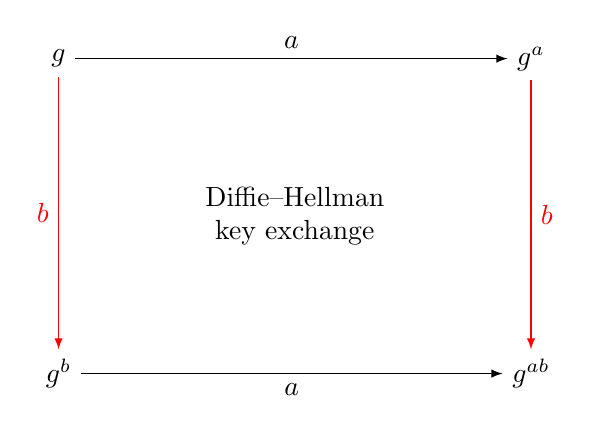
\begin{tikzpicture}
        \draw
        (0,0) node(g) {$g$}
        (6,0) node(ga) {$g^a$}
        (g) edge[-latex] node[above] {$a$} (ga);

        \uncover<2->{
          \draw
          (0,-4) node(gb) {$g^b$}
          (6,-4) node(gab) {$g^{ab}$}
          (gb) edge[-latex] node[below] {$a$} (gab);
          \draw[red]
          (g) edge[-latex] node[left] {$b$} (gb)
          (ga) edge[-latex] node[right] {$b$} (gab);
          \node[align=center] at (3,-2) {Diffie--Hellman\\key exchange};
        }
      \end{tikzpicture}
    \end{column}
  \end{columns}
\end{frame}

%%

\begin{frame}
  \centering
  \begin{tabular}{>{\centering\arraybackslash}m{0.5\textwidth} >{\centering\arraybackslash}m{0.5\textwidth}}
    \includegraphics[width=0.5\textwidth]{dh}
    & \uncover<2>{\includegraphics[width=0.4\textwidth]{shor}}\\
    \textit{Diffie--Hellman key exchange}
    & \uncover<2>{\textit{Shor's algorithm}}
  \end{tabular}
\end{frame}

%%

\begin{frame}
  \Large
  \begin{tikzpicture}[remember picture,overlay,shift={(current page.center)},xscale=0.5]
    \fill[white] (0,8) -- (16,8) -- (16,-8) -- (0,-8);
    \fill[ibmblue] (0,8) -- (-16,8) -- (-16,-8) -- (0,-8);
    
    \node[white,anchor=east] at (0,3.5) {\LARGE\bf Only two ways to};
    \node[ibmblue,anchor=west] at (0,3.5) {\LARGE\bf Post-quantum Encryption};
    
    \node[white,align=center] at (-8,0) {Noisy linear algebra:\\\normalsize Lattices, Codes};
    \node[ibmblue,align=center] at (8,0) {Far-fetched generalizations\\of the discrete logarithm:\\\normalsize Isogenies};
  \end{tikzpicture}
\end{frame}

%%

\begin{frame}{What crypto from isogenies?}
  
  \renewcommand{\arraystretch}{1.5}
  \begin{tabular}{l p{0.27\textwidth} p{0.27\textwidth} p{0.20\textwidth}}
    & \emph{Key exchange/Encryption} & \emph{Identification/Signature} & \emph{Other}\\
    \hline
    \emph{Group action}
    & Couveignes--Rostovtsev--Stolbunov\par CSIDH\par SCALLOP
                                & SeaSign\par CSI-FiSh\par PEGASIS
                                                             & Threshold\par PAKE\par \dots\\
    \emph{Groupoid action}
    & ---
                                & Galbraith--Petit--Silva\par \strut\emph{SQIsign}\par SIDH-like signatures
                                                             & Ring signatures\par Adaptor signatures\par \dots\\
    \emph{\textit{Ad hoc}}\footnote{see D., Fouotsa, Panny, \textit{``Isogeny problems with level structure''}, \url{https://ia.cr/2024/459}}
    & \strut\alert{SIDH~$\dagger$}\par SIDH fixes\par FESTA
                                & SIDH-like signatures
                                                             & Time-release crypto\par\dots
  \end{tabular}
\end{frame}

%%

\begin{frame}{What's needed for key exchange?}
  \begin{columns}
    \begin{column}{0.5\textwidth}
      \centering
      \begin{tikzpicture}
        \begin{uncoverenv}<-3>
          \begin{scope}
            \def\crater{13}
            \def\jumpa{-8}
            \def\diam{2.5cm}

            \uncover<1>{
              \foreach \i in {1,...,\crater} {
                \draw[blue!20!white] (360/\crater*\i : \diam) to[bend right] (360/\crater*\i+360/\crater : \diam);
              }
            }

            \uncover<2->{
              \pgfmathparse{int(\crater/2)}
              \let\last\pgfmathresult
              \foreach \i in {1,...,\last} {
                \pgfmathparse{mod(pow(2,\i-1),\crater)}
                \let\e\pgfmathresult
                \draw[red] (360/\crater*\e : \diam) to[bend left] (360/\crater*\e*2 : \diam);
                \draw[red] (-360/\crater*\e : \diam) to[bend right] (-360/\crater*\e*2 : \diam);
              }
            }

            \uncover<3->{
              \pgfmathparse{int(\crater/2)}
              \let\last\pgfmathresult
              \foreach \i in {1,...,\last} {
                \pgfmathparse{mod(pow(6,\i-1),\crater)}
                \let\e\pgfmathresult
                \draw[blue] (360/\crater*\e : \diam) to[bend right] (360/\crater*\e*6 : \diam);
                \draw[blue] (-360/\crater*\e : \diam) to[bend left] (-360/\crater*\e*6 : \diam);
              }
            }
            
            \pgfmathparse{\crater-1}
            \let\last\pgfmathresult
            \foreach \i in {0,...,\last} {
              \draw[fill] (360/\crater*\i: \diam) circle (2pt) +(360/\crater*\i: 0.5) node{$g^{\i}$};
            }
          \end{scope}
        \end{uncoverenv}
        
        \begin{uncoverenv}<4->
          \begin{scope}
            \def\crater{12}
            \def\jumpa{5}
            \def\diam{2.5cm}

            \foreach \i in {1,...,\crater} {
              \draw[red,-latex] (360/\crater*\i : \diam) to[bend right] (360/\crater*\i+360/\crater : \diam);
              \draw[blue,-latex] (360/\crater*\i : \diam) to[bend right=10] (360/\crater*\i+\jumpa*360/\crater : \diam);
            }

            \foreach \i in {1,...,\crater} {
              \pgfmathparse{int(mod(pow(2,\i-1),\crater+1))}
              \let\e\pgfmathresult
              \draw[fill] (360/\crater*\i: \diam) circle (2pt) +(360/\crater*\i: 0.5) node{$g^{\e}$};
            }
          \end{scope}
        \end{uncoverenv}
      \end{tikzpicture}
    \end{column}
    \begin{column}{0.4\textwidth}
      The axioms of a dlog group:
      \begin{itemize}
      \item[\sout{prod:}] \sout{$g^ag^b = g^{a+b}$,}
      \item[exp:] $(g^a)^b = g^{ab} = (g^b)^a$.
      \end{itemize}

      \bigskip
      The hard problem:
      \begin{itemize}
      \item[dlog:] $g^a \mapsto a$.
      \end{itemize}

      \bigskip
      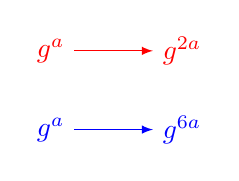
\begin{tikzpicture}
        \uncover<2->{\draw[red,-latex] (0,0) node[anchor=east]{$g^a$} -- (1,0) node[anchor=west] {$g^{2a}$};}
        \uncover<3->{\draw[blue,-latex] (0,-1) node[anchor=east]{$g^a$} -- (1,-1) node[anchor=west] {$g^{6a}$};}
      \end{tikzpicture}

      \bigskip
      \begin{uncoverenv}<5->
        Automorphism group: \emph{$(\Z/13\Z)^\times$}.
      \end{uncoverenv}
    \end{column}
  \end{columns}
\end{frame}

%%

\begin{frame}{Group action}
  \begin{columns}
    \begin{column}{0.5\textwidth}
      \emph{$\G\circlearrowright\E$}: A (finite) set $\E$ \emph{acted
        upon} by a group $\G$ \emph{freely} and \emph{transitively}:
      \begin{align*}
        * : \G × \E &→ \E\\
        \g * E &↦ E'
      \end{align*}
      \par\begin{description}
      \item[Compatibility:] \emph{$\g' * (\g * E) = (\g'\g)*E$} for all
        $\g,\g'\in\G$ and $E\in\E$;
      \item[Identity:] \emph{$\mathfrak{e} * E = E$} if and only if
        $\mathfrak{e}\in\G$ is the identity element;
      \item[Regularity:] for all $E,E'\in\E$ there exist a \emph{unique
          $\g\in\G$} such that \emph{$\g*E'=E$}.
        \setlength{\itemsep}{2em}
      \end{description}
    \end{column}
    \begin{column}{0.45\textwidth}
      \centering
      \begin{uncoverenv}<2->
        \emph{Example:} $(ℤ/13ℤ)^\ast \quad\circlearrowright\quad (C_{13} \setminus \{1\})$

        \bigskip
        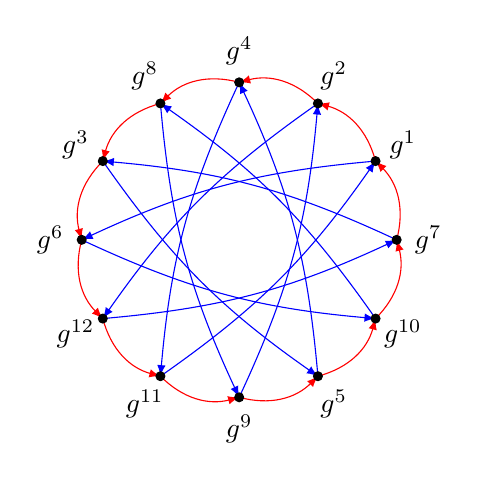
\begin{tikzpicture}[scale=0.8]
          \def\crater{12}
          \def\jumpa{5}
          \def\diam{2.5cm}

          \foreach \i in {1,...,\crater} {
            \draw[red,-latex] (360/\crater*\i : \diam) to[bend right] (360/\crater*\i+360/\crater : \diam);
            \draw[blue,-latex] (360/\crater*\i : \diam) to[bend right=10] (360/\crater*\i+\jumpa*360/\crater : \diam);
          }

          \foreach \i in {1,...,\crater} {
            \pgfmathparse{int(mod(pow(2,\i-1),\crater+1))}
            \let\e\pgfmathresult
            \draw[fill] (360/\crater*\i: \diam) circle (2pt) +(360/\crater*\i: 0.5) node{$g^{\e}$};
          }
        \end{tikzpicture}
      \end{uncoverenv}
    \end{column}
  \end{columns}
\end{frame}

%%

\begin{frame}{Cryptographic Group Actions}
  \footnotetext[1]{Couveignes 1997. \url{https://ia.cr/2006/291}}
  \footnotetext[2]{Alamati, D., Montgomery, Patranabis 2021. \url{https://ia.cr/2020/1188}}
  
  \large
  \begin{columns}
    \begin{column}{0.5\textwidth}
      %{Hard Homogeneous Space (HHS) ---  }
      \begin{description}
        \setlength{\itemsep}{1em}
      \item[Setup:] A group action \emph{$\G\circlearrowright\E$}\\
        \uncover<2->{\alert{with $\G$ commutative}}
      \item[Easy:] $E' \quad\mapsto\quad \g*E$\\{\small(evaluation)}
      \item[Hard:] $\g*E \quad\mapsto\quad \g$\\{\small(inversion)}
      \end{description}
    \end{column}
    \begin{column}{0.5\textwidth}
      \centering
      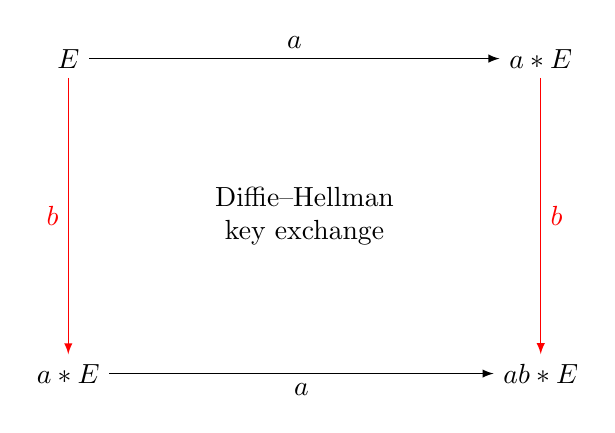
\begin{tikzpicture}
        \draw
        (0,0) node(g) {$E$}
        (6,0) node(ga) {$\a * E$}
        (g) edge[-latex] node[above] {$\a$} (ga);

        \uncover<2->{
          \draw
          (0,-4) node(gb) {$\a * E$}
          (6,-4) node(gab) {$\a\b * E$}
          (gb) edge[-latex] node[below] {$\a$} (gab);
          \draw[red]
          (g) edge[-latex] node[left] {$\b$} (gb)
          (ga) edge[-latex] node[right] {$\b$} (gab);
          \node[align=center] at (3,-2) {Diffie--Hellman\\key exchange};
        }
      \end{tikzpicture}
    \end{column}
  \end{columns}
\end{frame}

%%

\begin{frame}{\alert<2->{Cryptographic} Group Actions in the Wild}
  \large
  \begin{description}[labelwidth=0]
    \setlength{\itemsep}{2em}
  \item[Abelian]
    \begin{itemize}
    \item \alt<3->{\alert{\sout{Discrete logarithm}}}{Discrete logarithm}
    \item Isogenies:
      \begin{itemize}
      \item Complex multiplication (Couveignes--Rostovtsev--Stolbunov)
      \item $\pi$-oriented (CSIDH)
      \item Arbitrary orientations (SCALLOP, \dots)
      \end{itemize}
    \end{itemize}
  \item[Non-Abelian]
    \begin{itemize}
    \item Isomorphism of Codes (PCE, LCE)
    \item Lattice Isomorphism
    \item \alt<2->{\alert{\sout{Graph Isomorphism}}}{Graph Isomorphism}
    \end{itemize}
  \end{description}
\end{frame}

%%

\begin{frame}{Quantum security}
  \large
  \begin{center}
    \emph{Group Action Inversion $→$ Hidden Shift Problem}
  \end{center}

  \bigskip
  
  \begin{description}[labelwidth=0]
    \setlength{\itemsep}{2em}
  \item[Abelian:]
    \begin{itemize}
    \item Abelian Hidden Shift Problem $→$ Dihedral Hidden Subgroup
      Problem
    \item Kuperberg's algorithm (quantum subexponential time)
    \end{itemize}
  \item[Non-Abelian:]
    no quantum speedup known
  \end{description}
\end{frame}

%%

\begin{frame}{Zero-Knowledge Proofs of Knowledge (ZK-PoK)}
  \centering
  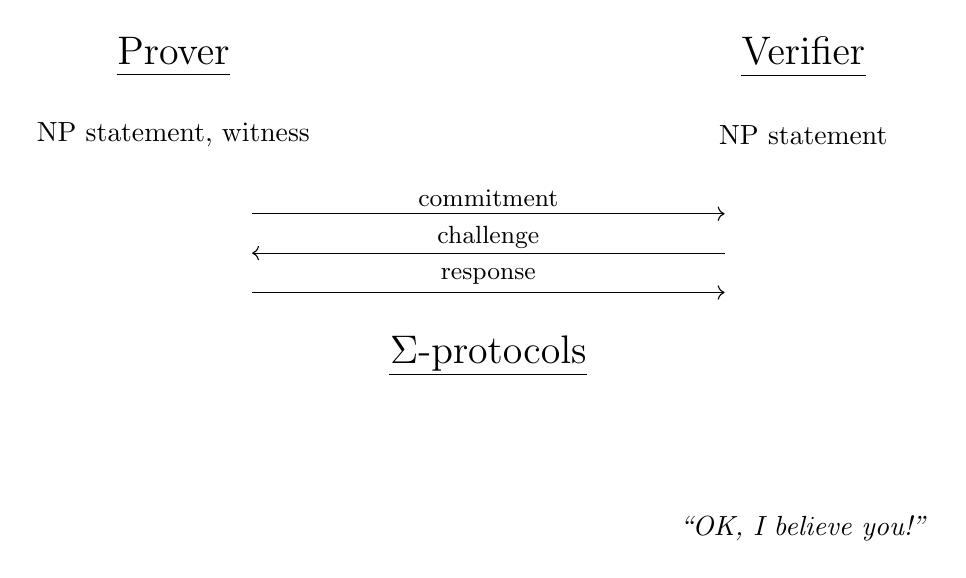
\begin{tikzpicture}
    \node at (0,0) {\Large\emph{Prover}};
    \node at (0,-1) {NP statement, witness};
    
    \node at (8,0) {\Large\emph{Verifier}};
    \node at (8,-1) {NP statement};

    \draw
    (1,-2) edge[->] +(6,0)
    ++(0,-0.5) edge[<-] +(6,0)
    ++(0,-0.5) edge[->] +(6,0);
      
    \node at (8, -6) {\textit{``OK, I believe you!''}};

    \draw
    (4,-1.8) node{\small commitment}
    ++(0,-0.5) node{\small challenge}
    ++(0,-0.5) node{\small response}
    ++(0,-1) node{\Large\emph{$\Sigma$-protocols}};
  \end{tikzpicture}
\end{frame}

%%

\begin{frame}{A ZK-PoK for Graph Isomorphism (after Goldwasser--Micali--Rackoff)}
  \begin{center}
    \begin{tikzpicture}
      \begin{scope}
        \Large
        \node (G) at (0,0) {$G$};
        \node (H) at (4,0) {$H$};

        \draw[->] (G) edge node[above]{$\sigma$} (H);

        \uncover<2->{
          \node (R) at (2,-3) {$R$};
        }
        \uncover<2>{
          \draw[->] (G) edge node[left]{$\pi$} (R);
        }

        \uncover<4->{
          \draw[->,dashed] (R) edge node[right]{$\sigma\circ\pi^{-1}$} (H);
          \draw[->,dashed] (R) edge node[left]{$\pi^{-1}$} (G);
        }
      \end{scope}

      \draw[gray] (6,1) -- ++(0,-5);
      
      \begin{scope}[xshift=8cm]
        \node at (0,0) {\emph{Prover}};
        \node at (4,0) {\emph{Verifier}};

        \uncover<2->{
          \draw[->] (0,-1) to node[above]{$R$} ++(4,0);
        }

        \uncover<3->{
          \draw[<-] (0,-2) to node[above]{$b\in\{0,1\}$} ++(4,0);
        }

        \uncover<4->{
          \draw[->] (0,-3) to node[above]{$\sigma^b\circ\pi^{-1}$} ++(4,0);
        }
      \end{scope}
    \end{tikzpicture}
  \end{center}

  \bigskip
  \begin{uncoverenv}<5->
    Basis for:
    \emph{SeaSign / CSI-FiSh} (isogenies),
    \emph{LESS} (codes)
  \end{uncoverenv}
\end{frame}

%%

\begin{frame}{Groupoids}
  \large

  \begin{columns}
    \begin{column}{0.7\textwidth}
      A groupoid is a non-empty set $\G$ with two operations
      \begin{description}
      \item[Inverse:] $^{-1} : \G \to \G$
      \item[Product:] a \emph{partial} function $\quad\cdot : \G × \G \rightharpoonup \G$
      \end{description}

      \bigskip
      And axioms
      \begin{description}[labelwidth=0]
      \item[Associativity:] \emph{$\a \cdot (\b \cdot \c) = (\a \cdot \b) \cdot \c$} if either is defined,
      \item[Inverse:] \emph{$\a \cdot \a^{-1}$} and \emph{$\a^{-1} \cdot \a$} are always defined,
      \item[Identity:] if $\a\cdot \b$ is defined \emph{$\a \cdot \b \cdot \b^{-1} = \a$} and
        \emph{$\a^{-1} \cdot \a \cdot \b = \b$}.
      \end{description}
    \end{column}
    \begin{column}{0.3\textwidth}
      \centering
      \begin{tikzpicture}
        \node (A) at (2,3) {$\bullet$};
        \node (B) at (0,0) {$\bullet$};
        \node (C) at (4,0) {$\bullet$};

        \draw[-latex]
        (A) edge node[left] {$\a$} (B)
        (A) edge node[right] {$\b$} (C)
        (B) edge node[below] {$\b \cdot \a^{-1}$} (C);
      \end{tikzpicture}
    \end{column}
  \end{columns}
\end{frame}

%%

\begin{frame}{Groupoid action}
  \large
  \begin{columns}
    \begin{column}{0.7\textwidth}
      \emph{$\G\circlearrowright\E$}: A (finite) set $\E$ \emph{acted
        upon} by a groupoid $\G$ \emph{freely} and \emph{transitively}:
      \begin{align*}
        * : \G × \E &\rightharpoonup \E\\
        \g * E &\mapsto E'
      \end{align*}
      \par\begin{description}[labelwidth=0]
      \item[Compatibility:] \emph{$\g' * (\g * E) = (\g'\g)*E$} whenever either is defined;
      \item[Identity:] \emph{$(\g^{-1}\g) * E = E$} whenever $\g * E$ is defined;
      \item[Regularity:] for all $E,E'\in\E$ there exist a \emph{unique
          $\g\in\G$} such that \emph{$\g*E'=E$}.
        \setlength{\itemsep}{2em}
      \end{description}
    \end{column}
    \begin{column}{0.3\textwidth}
      \centering
      \begin{tikzpicture}
        \node (A) at (2,3) {$A$};
        \node (B) at (0,0) {$B$};
        \node (C) at (4,0) {$C$};

        \draw[-latex]
        (A) edge node[left] {$\a$} (B)
        (A) edge node[right] {$\b$} (C)
        (B) edge node[below] {$\b \cdot \a^{-1}$} (C);
      \end{tikzpicture}
    \end{column}
  \end{columns}
\end{frame}

%%

\begin{frame}<4>{A ZK-PoK from Groupoid Actions}
  \begin{center}
    \begin{tikzpicture}
      \begin{scope}
        \Large
        \node (G) at (0,0) {$G$};
        \node (H) at (4,0) {$H$};

        \draw[->] (G) edge node[above]{$\sigma$} (H);

        \uncover<2->{
          \node (R) at (2,-3) {$R$};
        }
        \uncover<2>{
          \draw[->] (G) edge node[left]{$\pi$} (R);
        }

        \uncover<4->{
          \draw[->,dashed] (R) edge node[right]{$\sigma\circ\pi^{-1}$} (H);
          \draw[->,dashed] (R) edge node[left]{$\pi^{-1}$} (G);
        }
      \end{scope}

      \draw[gray] (6,1) -- ++(0,-5);
      
      \begin{scope}[xshift=8cm]
        \node at (0,0) {\emph{Prover}};
        \node at (4,0) {\emph{Verifier}};

        \uncover<2->{
          \draw[->] (0,-1) to node[above]{$R$} ++(4,0);
        }

        \uncover<3->{
          \draw[<-] (0,-2) to node[above]{$b\in\{0,1\}$} ++(4,0);
        }

        \uncover<4->{
          \draw[->] (0,-3) to node[above]{$\sigma^b\circ\pi^{-1}$} ++(4,0);
        }
      \end{scope}
    \end{tikzpicture}
  \end{center}

  \bigskip
  \emph{Galbraith--Petit--Silva 2016:} it works!!! \textcolor{gray}{\small\dots in a very special case and with lots of quirks}
\end{frame}

%%

\begin{frame}{Morphisms of elliptic curves}
  \Large
  \begin{description}
    \setlength{\itemsep}{4em}
  \item[Isogenies =] finite-kernel \textit{algebraic} group morphisms: \emph{$E \to E'$}
  \item[Endomorphisms =] isogenies \emph{$E \to E$}
  \end{description}
\end{frame}

%%

\begin{frame}{Isogenies: an example over $\F_{11}$}
  \centering
  \begin{tikzpicture}[scale=0.4]
    \begin{scope}
      \node[anchor=center] at (0,7) {$E \;:\; y^2 = x^3 + x$};

      \uncover<-1>{
        \draw[thin,gray] (0,-6) -- (0,6);
        \draw[thin,gray] (-6,0) -- (6,0);
      }

      \foreach \x/\y in {0/0,5/3,-4/3,-3/5,-2/1,-1/3} {
        \draw[blue,fill] (\x,\y) circle (0.2) node(E_\x_\y){}
        (\x,-\y) circle (0.2) node(E_\x_-\y){};
      }

      \uncover<2->{\draw[red,fill] (0,0) circle (0.3);}
    \end{scope}

    \draw[black!10!white,thick] (10,-7) -- +(0,14);
    
    \begin{scope}[shift={(20,0)}]
      \node at (0,7) {$E' \;:\; y^2 = x^3 - 4x$};

      \uncover<-1>{
        \draw[thin,gray] (0,-6) -- (0,6);
        \draw[thin,gray] (-6,0) -- (6,0);
      }

      \foreach \x/\y in {0/0,2/0,3/2,4/2,6/4,-2/0,-1/5} {
        \draw[color=blue,fill] (\x,\y) circle (0.2) node(F_\x_\y){}
        (\x,-\y) circle (0.2) node(F_\x_-\y){};
      }
    \end{scope}

    \begin{scope}[color=red,-latex,dashed]
      \begin{uncoverenv}<2->
        \path
        (E_5_3) edge (F_3_2)
        (E_-4_3) edge (F_4_-2)
        (E_-3_5) edge (F_4_2)
        (E_-2_1) edge (F_3_-2)
        (E_-1_3) edge (F_-2_0);
      \end{uncoverenv}
      \begin{uncoverenv}<2->
        \path
        (E_5_-3) edge (F_3_-2)
        (E_-4_-3) edge (F_4_2)
        (E_-3_-5) edge (F_4_-2)
        (E_-2_-1) edge (F_3_2)
        (E_-1_-3) edge (F_-2_0);
      \end{uncoverenv}
    \end{scope}
  \end{tikzpicture}
  
  \begin{columns}
    \begin{column}{0.5\textwidth}
      \[\phi(x,y) = \left(\frac{x^2 + 1}{x},\quad y\frac{x^2-1}{x^2}\right)\]
    \end{column}
    \begin{column}{0.5\textwidth}
      \begin{itemize}
      \item<2-> Kernel generator in \alert{red}.
      \item<2-> This is a degree $2$ map.
      \item<2-> Analogous to $x\mapsto x^2$ in $\F_q^*$.
      \end{itemize}
    \end{column}
  \end{columns}
\end{frame}

%%

\begin{frame}{Degree and dual}
  \large
  Let \emph{$φ : E \to E'$}. There exist:

  \smallskip
  \begin{uncoverenv}<2->
    \begin{description}
    \item[Degree:] a smallest integer \emph{$d > 0$}, and
    \item[Dual:] a unique isogeny \emph{$\widehat{φ} : E' \to E$},
    \item<3-> such that:
    \end{description}
  \end{uncoverenv}
  
  \medskip
  \centering
  \begin{tikzpicture}
    \node (E1) at (6,0) {$E'$};
    \node (E) at (0,0) {$E$};

    \draw[-latex] (E) edge[bend left] node[above] {$φ$} (E1);

    \uncover<2->{
      \draw[-latex] (E1) edge[bend left] node[below] {$\widehat{φ}$} (E);
    }
    
    \uncover<3->{
      \draw[-latex] (E1) edge[loop,out=45,in=-45,looseness=10] node[right] {mul.\ by $d$} (E1);
      \draw[-latex] (E) edge[loop,out=135,in=225,looseness=10] node[left] {mul.\ by $d$} (E);
    }
  \end{tikzpicture}
\end{frame}

%%

\begin{frame}{Anatomy of an isogeny}
  \transdissolve<2-8>
  \large
  \centering
  \begin{tikzpicture}
    \node at (-6,0) {$\phi(x,y) = \Biggl($};
    \node (x) at (-2.5,0) {$\displaystyle
      \frac{
        \only<-6>{x^4 - x^3 + 11x^2 + 9x + 12}
        \only<7->{g(x)}
      }{
        \only<-3>{\phantom{(}x^3-x^2-x+1\phantom{)}}
        \only<4-5>{(x + 1)(x - 1)^2}
        \only<6->{h(x)}
      },$};
    \node (y) at (3.5,0) {$\displaystyle y
      \only<-7>{\frac{x^5 - x^4 - 14x^3 - 26x^2 - 67x - 21}{x^5 - x^4 - 2x^3 + 2x^2 + x - 1}}
      \only<8->{\left(\frac{g(x)}{h(x)}\right)'}$};
    \node at (7,0) {$\Biggr)$};
    
    \begin{scope}[thick,red]
      \uncover<2-6>{\draw (-4.5,0.4) circle (0.2) +(0,0.2) -- +(0,1) +(0,1.2) node {degree};}
      \uncover<2>{\draw (-3.6,-0.2) circle (0.2) +(0,-0.2) -- +(0,-1) +(0,-1.2) node {degree $-1$};}
      \uncover<3-4>{
        \draw (-2.5,-0.3) ellipse (1.7 and 0.4) +(0,-0.4) -- +(0,-1.2) +(0,-1.4) node {kernel polynomial};
      }
      \uncover<5>{
        \draw (-3.3,-0.3) ellipse (0.7 and 0.4) +(-0.5,-0.3) -- +(-1,-0.6) +(-1.2,-0.8) node {Point of order $2$};
        \draw (-1.9,-0.3) ellipse (0.9 and 0.4) +(0.2,-0.4) -- +(1,-1.5) +(1.1,-1.7) node {Two points of order $4$};
      }
      \uncover<6->{
        \draw (-2.5,-0.6) -- +(0,-1) +(0,-1.5) node {$h(x) = \displaystyle\prod_{P\in K\setminus\{0\}}\bigl(x-x(P)\bigr)$};
      }
      \uncover<7->{
        \draw (-2.5,0.6) -- +(0,1) +(0,1.5) node {computed by Vélu--Elkies--Kohel formulas};
      }
    \end{scope}
  \end{tikzpicture}

  \medskip
  
  \begin{uncoverenv}<9->
    \begin{description}
    \item[Input:] Finite kernel \emph{$K⊂E$} of order \emph{$d$};
    \item[Output:] Rational fractions \emph{$ϕ(x,y)$};
    \item[Complexity:] \emph{$\tilde{O}(d)$} operations.
    \end{description}
  \end{uncoverenv}
\end{frame}

%%

\begin{frame}{How many isogenies?}
  \large
  \begin{tikzpicture}
    \node (K) at (-4, 0) {
      \begin{minipage}{6cm}
        \centering
        Finite subgroups of order $d$
        \[\emph{K ⊂ E}\]
      \end{minipage}
    };
    \node (I) at (4, 0) {
      \begin{minipage}{6cm}
        \centering
        Isogenies of degree $d$
        \[\emph{\phi: E \to E/K}\]
        {\normalsize (up to composing with isomorphism)}
      \end{minipage}
    };
    \draw[latex-latex] (K) edge (I);
  \end{tikzpicture}

  \pause
  \vfill

  \emph{Examples:}

  \begin{table}
    \begin{tabular}{l l}
      If $d$ is prime &$→$ at most \emph{$d+1$} possible kernels,\\[0.5em]
      In general      &$→$ at most \emph{$≈ d$} possible kernels.
    \end{tabular}
  \end{table}
\end{frame}

%%

\begin{frame}{The isogeny one-way function}
  \large
  \begin{columns}
    \begin{column}{0.5\textwidth}
      \begin{description}
        \setlength{\itemsep}{1em}
      \item[Setup:] A class of isogenous curves
      \item[Easy:] $E,K \quad\mapsto\quad E/K$
      \item[Hard:] $E,E/K \quad\mapsto\quad K$
      \end{description}
    \end{column}
    \begin{column}{0.5\textwidth}
      \centering
      \begin{tikzpicture}
        \draw
        (0,0) node(g) {$E$}
        (6,0) node(ga) {$E'$}
        (g) edge[-latex] node[above] {??} (ga);
      \end{tikzpicture}
    \end{column}
  \end{columns}
\end{frame}

%%

\begin{frame}
  \huge\centering
  Do isogenies form a groupoid?
\end{frame}

%%

\begin{frame}{Lattices of isogenies}
  \centering
  \begin{tikzpicture}
    \large
    \node (E1) at (0,0) {$E'$};
    \node (E) at (6,0) {$E$};
    \uncover<2->{
      \draw[dashed,->] (E) edge node[above]
      {$\uncover<3->{\alert{a}}φ+\uncover<3->{\alert{b}}ψ$} (E1);
    }
    
    \draw[->] (E) edge[bend right] node[above] {$φ$} (E1)
    edge[bend left] node[above] {$ψ$} (E1);
    \node at (9,1) {$φ,ψ ∈ \Hom(E,E')$};
    \uncover<3->{
      \node at (12,1) {\alert{$a,b∈ℤ$}};
    }

    \uncover<2->{
      \node at (10,-1) {$(\uncover<3->{\alert{a}}φ + \uncover<3->{\alert{b}}ψ)(P)
        :=
        \uncover<3->{[\alert{a}]}φ(P) + \uncover<3->{[\alert{b}]}ψ(P)$};
    }
  \end{tikzpicture}

  \bigskip
  
  \uncover<4->{
    \begin{itemize}
      \setlength{\itemsep}{1.5em}
    \item $\deg(aφ) = a^2\deg(φ)$,
    \item $\big\lvert \deg(φ+ψ) - \deg(φ) - \deg(ψ) \big\rvert ≤ 2\sqrt{\deg(φ)\deg(ψ)}$,
    \item $\deg$ is a \emph{positive definite quadratic form.}
    \end{itemize}
  }
\end{frame}

%%

\begin{frame}{Endomorphism rings}
  \large
  \begin{itemize}
    \setlength{\itemsep}{2em}
  \item $\Hom(A,B)$: additive group
  \item Distributivity:
    \begin{align*}
      φ∘(ψ+χ) &= (φ∘ψ)+(φ∘χ)\\[2em]
      (ψ+χ)∘φ &= (ψ∘φ)+(χ∘φ)\\
    \end{align*}
  \item It follows that \emph{$\End(A) := \Hom(A,A)$} is a ring.
  \end{itemize}  
\end{frame}

%%

\begin{frame}{Endomorphism rings}
  \large $\End(E)$ is a free $ℤ$-module of rank \textcolor{blue}{1},
  \textcolor{purple}{2} or \textcolor{red}{4}. As a ring:

  \bigskip
  \begin{enumerate}
    \setlength{\itemsep}{1em}
  \item[\color{blue}1)] $\End(E) ≃ ℤ$;
  \item[\color{purple}2)] $\End(E) ⊂$ quadratic imaginary field;
  \item[\color{red}4)] $\End(E) ⊂$ quaternion algebra.
  \end{enumerate}
\end{frame}

%%

\begin{frame}{Isogenies = $\End(E)$-Ideals}
  \large\centering
  \begin{tikzpicture}
    \node (E1) at (0,0) {$E'$};
    \node (E) at (6,0) {$E$};

    \draw[-latex] (E) edge node[above] {$φ$} (E1);
    \uncover<1>{
      \node at (3,-3) {$φ ∈ \Hom(E,E')$};
    }

    \uncover<2>{
      \draw[-latex] (E) edge[loop,out=45,in=-45,looseness=10] node[right] {$ω$} (E);
      \node at (3,-3) {$φ∘ω ∈ \Hom(E,E')$};
    }
    
    \uncover<3>{
      \draw[-latex] (E1) edge[loop,out=135,in=225,looseness=10] node[left] {$ω'$} (E1);
      \node at (3,-3) {$ω'∘φ ∈ \Hom(E,E')$};
    }
  \end{tikzpicture}
\end{frame}

%%

\begin{frame}{The Deuring correspondence: Isogenies $\longleftrightarrow$ Ideals}
  \large $\Hom(E,E')$ is a free $ℤ$-module of rank
  \textcolor{blue}{1}, \textcolor{purple}{2} or \textcolor{red}{4}.

  \bigskip
  It is a \emph{rank-1} projective $\End(E)$-module, isomorphic to:

  \bigskip
  \begin{enumerate}
    \setlength{\itemsep}{1em}
  \item[\color{blue}1)] an ideal of \textcolor{blue}{$ℤ$};
  \item[\color{purple}2)] an invertible ideal of a
    \textcolor{purple}{quadratic imaginary field};
  \item[\color{red}4)] an invertible ideal of a
    \textcolor{red}{quaternion algebra}.
  \end{enumerate}

  \bigskip
  As a quadratic module: \emph{degree $\longleftrightarrow$ norm}
\end{frame}

%%

\begin{frame}{The Deuring correspondence: Isogenies $\longleftrightarrow$ Ideal classes}
  \Large
  \begin{description}
    \setlength{\itemsep}{2em}
  \item[Equivalent ideals:]
    \[I ≃ J  \quad\Longleftrightarrow\quad I = Jα\]
  \item[Deuring correspondence:]
    \[\Hom(E,E') \quad\longleftrightarrow\quad \mathrm{cls}(I)\]
  \end{description}
  
  \bigskip \emph{Fact:} the ideal classes \emph{$\mathrm{cls}(I)$ form a groupoid!}
\end{frame}

%% 

\begin{frame}{Two computational worlds}
  \centering
  \setlength{\tabcolsep}{2em}
  \renewcommand{\arraystretch}{1.5}
  \begin{tabular}{p{0.3\textwidth} c c}
    & \textcolor{purple}{Quadratic imaginary} & \textcolor{red}{Quaternionic}\\
    \hline
    $\rank\Hom(E,E')$ & 2 & 4\\
    Endomorphism algebra & number field & quaternion algebra\\
    Maximal orders & one & many \\
    Ideal class\dots & \dots group & \dots groupoid\\
    Find isogeny $E → E'$ & \alert{hard} & \alert{hard}\\
    Convert isogenies $\leftrightarrow$ ideals & easy\footnotemark[1] & easy\footnote[1]{When $\End(E)$ is known}\\
    Compute $\End(E)$ & easy & \alert{hard}\\
  \end{tabular}
\end{frame}

%%

\begin{frame}{The quadratic imaginary case}
  \begin{block}{Complex Multiplication}
    Fix an order \emph{$\O ⊂ ℚ(\sqrt{-D})$}:
    \begin{itemize}
    \item Invertible ideal classes form a \emph{finite abelian group}
    \item $\Cl(\O)$ acts \emph{freely and transitively} on the set of
      elliptic curves with $\End(E) ≃ \O$.
    \end{itemize}
  \end{block}
\end{frame}

%%

\begin{frame}{What crypto from isogenies?}
  
  \renewcommand{\arraystretch}{1.5}
  \begin{tabular}{l p{0.27\textwidth} p{0.27\textwidth} p{0.20\textwidth}}
    & \emph{Key exchange/Encryption} & \emph{Identification/Signature} & \emph{Other}\\
    \hline
    \emph{Group action}
    & Couveignes--Rostovtsev--Stolbunov\par CSIDH\par SCALLOP
                                & SeaSign\par CSI-FiSh\par PEGASIS
                                                             & Threshold\par PAKE\par \dots\\
    \emph{Groupoid action}
    & ---
                                & Galbraith--Petit--Silva\par \strut\emph{SQIsign}\par SIDH-like signatures
                                                             & Ring signatures\par Adaptor signatures\par \dots\\
    \emph{\textit{Ad hoc}}\footnote{see D., Fouotsa, Panny, \textit{``Isogeny problems with level structure''}, \url{https://ia.cr/2024/459}}
    & \strut\alert{SIDH~$\dagger$}\par SIDH fixes\par FESTA
                                & SIDH-like signatures
                                                             & Time-release crypto\par\dots
  \end{tabular}
\end{frame}

%%

\begin{frame}{Two computational worlds}
  \centering
  \setlength{\tabcolsep}{2em}
  \renewcommand{\arraystretch}{1.5}
  \begin{tabular}{p{0.3\textwidth} c c}
    & \textcolor{purple}{Quadratic imaginary} & \textcolor{red}{Quaternionic}\\
    \hline
    $\rank\Hom(E,E')$ & 2 & 4\\
    Endomorphism algebra & number field & quaternion algebra\\
    Maximal orders & one & many \\
    Ideal class\dots & \dots group & \dots groupoid\\
    Find isogeny $E → E'$ & \alert{hard} & \alert{hard}\\
    Convert isogenies $\leftrightarrow$ ideals & easy\footnotemark[1] & easy\footnote[1]{When $\End(E)$ is known}\\
    Compute $\End(E)$ & easy & \alert{hard}\\
  \end{tabular}
\end{frame}

%%

\begin{frame}{The quaternionic case}
  \large
  \begin{itemize}
    \setlength{\itemsep}{2em}
  \item A supersingular curve,
  \item with an explicit basis of $\End(E_0)$,
  \item and an explicit embedding of $\End(E_0)$ in a quaternion algebra,
  \end{itemize}

  \bigskip
  \pause

  \begin{block}{The endomorphism ring problem
      \uncover<3->{\alert{\dots can be solved for a handful of curves!}}}
    Given a random supersingular curve $E/\F_{p^2}$, compute $\End(E)$.
  \end{block}
\end{frame}

%%

\begin{frame}{Contagious knowledge}
  \centering
  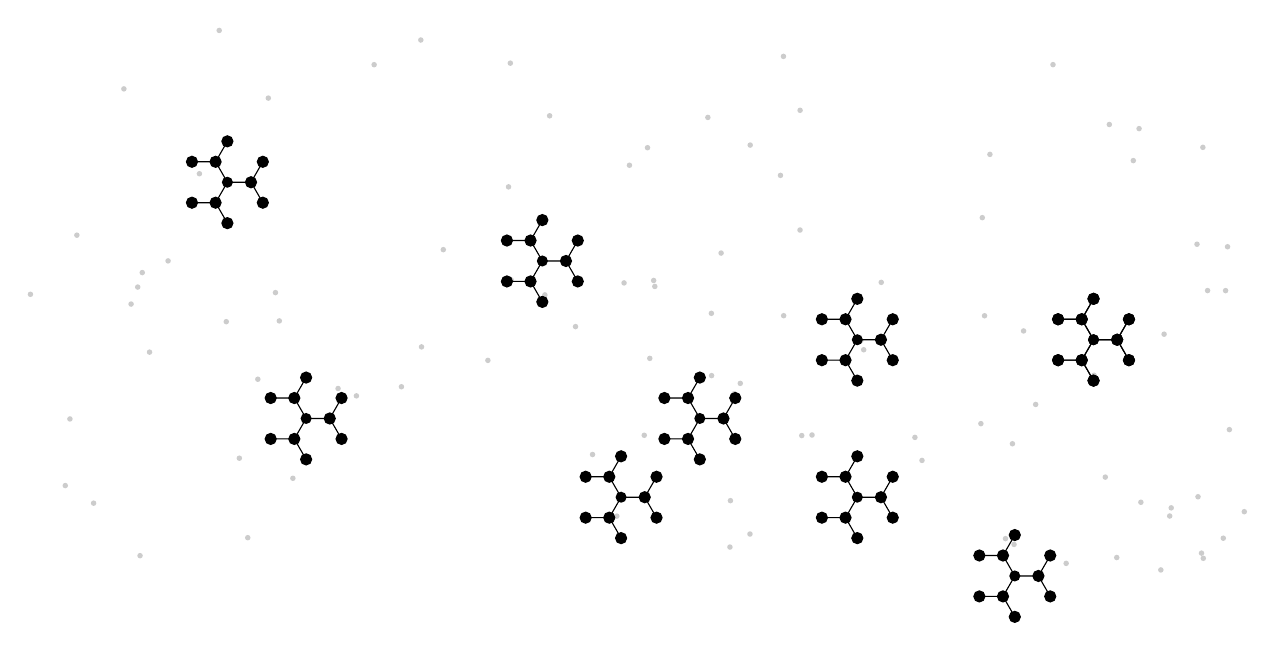
\begin{tikzpicture}
    \pgfmathsetseed{12345}
    \foreach \i in {1,...,100} {
      \pgfmathparse{16*random()}
      \let\x\pgfmathresult
      \pgfmathparse{7*random()}
      \let\y\pgfmathresult
      \fill[black!20!white] (\x,\y) circle (1pt);
    }
    \foreach \i in {1,...,10} {
      \pgfmathparse{floor(15*random())}
      \let\x\pgfmathresult
      \pgfmathparse{floor(6*random())}
      \let\y\pgfmathresult
      \fill (\x,\y) circle (2pt);
      \uncover<2->{
        \foreach \rho in {0,1,2} {
          \draw[fill,-latex] (\x,\y) -- +(120*\rho:.3) circle (2pt);
          \uncover<3->{
            \foreach \sigma in {-1,1} {
              \draw[fill,-latex] (\x,\y) ++(120*\rho:.3) -- ++(120*\rho+60*\sigma:.3) circle (2pt);
            }
          }
        }
      }
    }
  \end{tikzpicture}
\end{frame}

%%

\begin{frame}{SQIsign (D.--Kohel--Leroux--Petit--Wesolowski 2020)}
  \transdissolve<4,6>
  \large
  \centering
  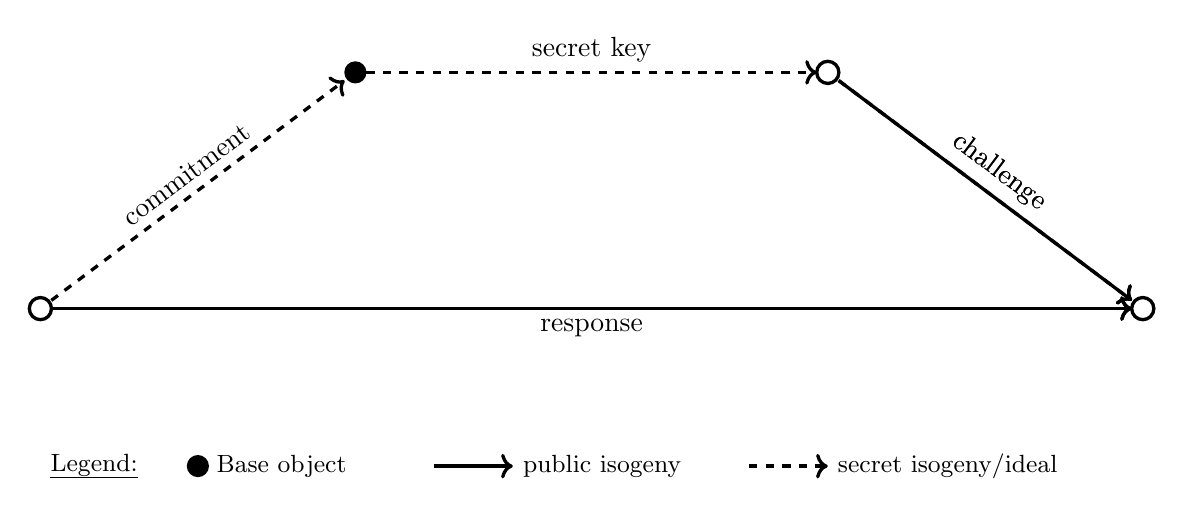
\begin{tikzpicture}[very thick]
    \fill
    (0,3) node(E0){} circle (4pt);
    \draw
    (6,3) node(PK){} circle (4pt);
    \draw[dashed,->] (E0) edge node[above,sloped] {secret key} (PK);
    
    \uncover<2->{
      \draw (-4,0) node(COM){} circle (4pt);
      \draw[dashed,->] (COM) edge node[sloped,above] {commitment} (E0);
    }

    \uncover<3->{
      \draw (10,0) node(CH){} circle (4pt);
    }
    \uncover<3,6->{
      \draw (PK) edge[->] node[sloped,above] {challenge} (CH);
    }

    \uncover<4-5>{
      \draw (PK) edge[dashed,->] node[sloped,above] {challenge} (CH);
    }

    \uncover<5>{
      \draw (COM) edge[dashed,->] (CH);
    }

    \uncover<6->{
      \draw (COM) edge[->] node[below] {response} (CH);
    }

    \begin{scope}[shift={(-4,-2)},anchor=west]
      \small
      \node at (0,0) {\emph{Legend:}};
      \fill (2,0) node(E0){~Base object} circle (4pt);
      \draw[->] (5,0) to ++(1,0) node {public isogeny};
      \draw[->,dashed] (9,0) to ++(1,0) node {secret isogeny/ideal};
    \end{scope}
  \end{tikzpicture}
\end{frame}

%%

\begin{frame}{Performance of SQIsign}

  \centering

  \textbf{SQIsign v1 (June 2023)}
  \begin{table}[h]
    \centering
    \begin{tabular}{c r r r r r}
      \toprule
      & \multicolumn{2}{c}{Sizes (bytes)} & \multicolumn{3}{c}{Timings (ms)}\\
      \cmidrule(lr){2-3}\cmidrule(lr){4-6}
        Security & Public Key & Signature & Keygen & Sign & Verify \\
      \midrule
        NIST-1 &  64 & 177 &  1,864 &  2,890 &    54 \\
        NIST-3 &  96 & 263 & 11,867 & 21,880 &   327 \\
        NIST-5 & 128 & 335 & 45,525 & 79,272 & 1,089 \\
      \midrule
    \end{tabular}
  \end{table}

  \vspace{.5em}
  \textbf{SQIsign v2 (June 2025)}
  \begin{table}[h]
    \centering
    \begin{tabular}{c r r r r r}
      % \toprule
      % & \multicolumn{2}{c}{\phantom{Sizes (bytes)}} & \multicolumn{3}{c}{\phantom{Timings (ms)}}\\[-2em]
      % \cmidrule(lr){2-3}\cmidrule(lr){4-6}
      \phantom{Security} & \phantom{Public Key} & \phantom{Signature} & \phantom{Keygen} & \phantom{Sign} & \phantom{Verify} \\[-2em]
      \midrule
        NIST-1 &  66 & 148 &  25 &   60 &  3 \\
        NIST-3 &  98 & 222 &  67 &  161 &  9 \\
        NIST-5 & 130 & 294 & 119 &  300 & 18 \\
      \bottomrule
    \end{tabular}
  \end{table}
\end{frame}

%%

\begin{frame}[plain]
  \centering
  \begin{tikzpicture}[remember picture,overlay]
    \begin{scope}[xscale=1.7,yshift=-15,opacity=0.8]
      \def\crater{12}
      \def\jumpa{-8}
      \def\jumpb{9}
      \def\diam{5cm}

      \foreach \i in {1,...,\crater} {
        \draw[blue] (360/\crater*\i : \diam) to[bend right] (360/\crater*\i+360/\crater : \diam);
        \draw[red] (360/\crater*\i : \diam) to[bend right] (360/\crater*\i+\jumpa*360/\crater : \diam);
        \draw[green] (360/\crater*\i : \diam) to[bend right=50] (360/\crater*\i+\jumpb*360/\crater : \diam);
      }
    \end{scope}
    
    \draw (0,0.5) node{\Huge\bf Thank you};
    \draw (0,-0.6) node{\large\url{https://defeo.lu/}};
    \draw (0,-1.3) node{\large\includegraphics[height=0.9em]{mastodon.png}~\href{https://twitter.com/luca_defeo}{@luca\_defeo@ioc.exchange}};
    \draw (0,-1.9) node{\large\includegraphics[height=0.9em]{bluesky.png}~\href{https://bsky.app/profile/bsky.defeo.lu}{@bsky.defeo.lu}};
  \end{tikzpicture}
\end{frame}

\end{document}


% LocalWords:  Isogeny abelian isogenies hyperelliptic supersingular Frobenius
% LocalWords:  isogenous
